\documentclass{beamer}
\usepackage{caption}
\usepackage{float}
\usepackage{lscape}
\usepackage{graphicx}% http://ctan.org/pkg/graphicx
\usepackage{booktabs}% http://ctan.org/pkg/booktabs
\usepackage{array}
\usepackage[export]{adjustbox}
\usepackage{amsmath}
\usepackage{amsfonts}
\usepackage{amssymb}
\usepackage{tikz}
\usepackage{ upgreek }
\usepackage{subcaption}
\usepackage{tabularx} 
\usepackage{setspace}





% version as of 10.26 2/24/19

\graphicspath{ {images/} }
\usetheme{Madrid}
\definecolor{Gold}{RGB}{218,165,32}
\setbeamertemplate{navigation symbols}{}
\setbeamertemplate{theorems}[numbered]
\setbeamertemplate{theorems}[ams style] 
\renewcommand{\qedsymbol}{$\blacksquare$}

\makeatletter

\setbeamerfont{footline}{size=\fontsize{6.5}{8.5}\selectfont}

\defbeamertemplate*{footline}{Dan P theme}
{
  \leavevmode%
  \hbox{%
  \begin{beamercolorbox}[wd=.15\paperwidth,ht=2.25ex,dp=1ex,center]{author in head/foot}%
    \usebeamerfont{author in head/foot}\insertshortauthor\expandafter\beamer@ifempty\expandafter{\beamer@shortinstitute}{}{~~(\insertshortinstitute)}
  \end{beamercolorbox}%
  \begin{beamercolorbox}[wd=.62\paperwidth,ht=2.25ex,dp=1ex,center]{title in head/foot}%
    \usebeamerfont{title in head/foot}\insertshorttitle
  \end{beamercolorbox}%
  \begin{beamercolorbox}[wd=.23\paperwidth,ht=2.25ex,dp=1ex,right]{date in head/foot}%
    \usebeamerfont{date in head/foot}\insertshortdate{}\hspace*{1.5em}
\insertframenumber{} / \inserttotalframenumber\hspace*{4ex} 
  \end{beamercolorbox}}%
  \vskip0pt%
}
\makeatother

\title{Cross-Industry Dispersion and the Cross-Section of Expected Returns \\ (Pinchuk 2019)}

% A subtitle is optional and this may be deleted
%\subtitle{Optional Subtitle}

\author{Mykola Pinchuk}

\date{09/22/2019}

\subject{Empirical Asset Pricing}

\AtBeginSubsection[]

\begin{document}

\begin{frame}
  \titlepage
\end{frame}


\begin{frame}{Introduction}
\begin{itemize}
    \item {The sectoral composition of the economy is permanently evolving.}
    \item {Many high-skill occupations (e.g., aerospace engineer) are specific to few industries.}
    \item {A decline of some industry creates unemployment risk for industry-specific occupations.}
    \item {Usually, industry-specific jobs are high-skill jobs.}
    \item {Complete hedging of labor income risk is impossible.}
    \item {Risk of losing these jobs should be relevant for asset pricing.}
\end{itemize}
\end{frame}



\begin{frame}{Idea and key results} \\
\textbf{Is the intensity of sectoral shifts a priced state variable?}
\vspace{0.64cm}
\begin{itemize}
    \item {I use Cross-Industry Dispersion (CID) to measure sectoral shifts.}
    \item {Stocks with high sensitivity to sectoral shifts deliver 8.5\% smaller returns than the stocks with low sensitivity.}
    \item {This return spread is not explained by common factors.}
    \item {CID spread can be a premium for unemployment risk due to sectoral shifts.}
    \item {Consistent with labor risk story, CID premium predicts unemployment.}
\end{itemize}
\end{frame}


\begin{frame}{Literature}
\begin{itemize}
    \item {Constantinides and Duffie (1996): In the model with heterogeneous agents, subject to uninsurable consumption shocks, cross-sectional variance of individual consumption growth is a state variable.}
    \item {Loungani, Rush and Tave (1990), Brainard and Cutler (1993): stock market dispersion index (very similar to CID) measures sectoral reallocation and predicts unemployment.}
    \item {Verousis and Voukelatos (2018): high sensitivity to Cross-Sectional Dispersion (CSD) predicts low returns due to idiosyncratic risk. }
\end{itemize}
\end{frame}


\begin{frame}{Data and CID}
\begin{itemize}
    \item {Sample: CRSP and Compustat 1963-2018.}
    \item {Cross-Industry Dispersion (CID) is the mean absolute deviation of the returns of FF49 industries.}
    \item {CID is measured at daily frequency.}
    $$CID_t = [\frac{1}{N}\sum^{N}_{i=1}{|R_i-R_{MKT}|}]_t$$
\end{itemize}
\end{frame}



\begin{frame}{Cross-sectional dispersion measures}
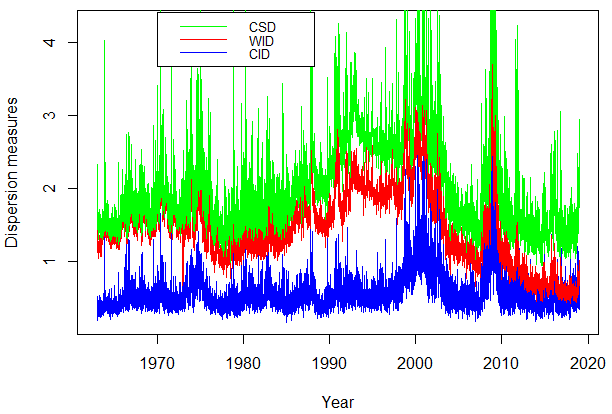
\includegraphics[width=1\textwidth]{cidwid.png}
\end{frame}



\begin{frame}{CID spread}
\begin{itemize}
    \item {I estimates $\beta_{CID}$ using 2 years of daily data}
    \item {I sort the stocks into decile portfolios by $\beta_{CID}$ and rebalance them monthly.}
\end{itemize}
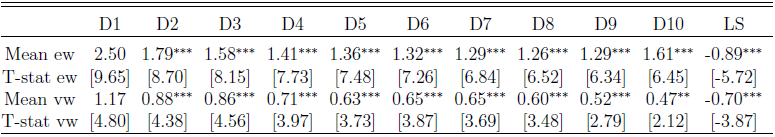
\includegraphics[width=1\textwidth]{table_spread.png}
\\
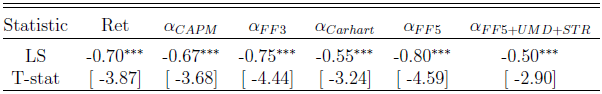
\includegraphics[width=1\textwidth]{abnormal_spread.png}
\end{frame}



\begin{frame}{CID spread and other variables}

% Table created by stargazer v.5.2.2 by Marek Hlavac, Harvard University. E-mail: hlavac at fas.harvard.edu
% Date and time: Tue, Sep 03, 2019 - 1:47:48 PM
\begin{table}[!htbp] \centering 
  \caption{\textbf{Abnormal returns of 5x5 portfolios, double-sorted on within-industry dispersion $\beta_{WID}$ and $\beta_{CID}$}} 
  \label{} 
  \footnotesize
\begin{tabular}{@{\extracolsep{2pt}} ccccccc} 
\\[-1.8ex]\hline 
\hline \\[-1.8ex] 
Statistic & Ret & $\alpha_{CAPM}$ & $\alpha_{FF3}$ & $\alpha_{Carhart}$ & $\alpha_{FF5}$ & $\alpha_{FF5+UMD+STR}$ \\ 
\hline \\[-1.8ex] 
L/S WID & 0.13 & 0.22 & 0.09 & -0.03 & -0.16 & -0.19 \\ 
T-stat & [ 0.89] & [ 1.46] & [ 0.61] & [ -0.19] & [ -1.08] & [ -1.27] \\ 
L/S CID & 0.38$^{***}$ & 0.34$^{**}$ & 0.44$^{***}$ & 0.38$^{***}$ & 0.59$^{***}$ & 0.43$^{***}$ \\ 
T-stat & [ 2.75] & [ 2.33] & [ 3.16] & [ 2.72] & [ 4.27] & [ 3.06] \\ 
\hline \\[-1.8ex] 
\end{tabular} 
\end{table}

\end{frame}



\begin{frame}{CID spread at lower frequencies}

% Table created by stargazer v.5.2.2 by Marek Hlavac, Harvard University. E-mail: hlavac at fas.harvard.edu
% Date and time: Mon, Sep 02, 2019 - 10:52:22 AM
\begin{table}[!htbp] \centering 
  \caption{\textbf{Returns of decile $\beta_{CID}$-sorted portfolios at different frequencies}} 
  \label{} 
  \setlength{\tabcolsep}{0pt} 
  \scriptsize

\begin{tabularx}{\linewidth}{p{2cm}p{1.2cm}p{1.2cm}p{1.2cm}p{1.2cm}p{1.2cm}p{1.2cm}}
    \toprule
    \multicolumn{7}{l}{\textbf{Panel A2: Quarterly abnormal returns of $\beta_{CID}$-sorted value-weighted portfolios}} \\
    \midrule
\\[-1.8ex]\hline 
\hline \\[-1.8ex] 
Statistic & Ret & $\alpha_{CAPM}$ & $\alpha_{FF3}$ & $\alpha_{Carhart}$ & $\alpha_{FF5}$ & $\alpha_{FF5+UMD+STR}$ \\ 
\hline \\[-1.8ex] 
LS Return & -1.29^{**} & -1.10^{*} & -1.60^{***} & -0.89^{} & -2.07^{***} & -1.16^{*} \\ 
T-stat & [ -2.30] & [ -1.95] & [ -2.91] & [ -1.56] & [ -3.63] & [ -1.90] \\ 
\hline \\[-1.8ex] 
\end{tabularx} 

\begin{tabularx}{\linewidth}{p{2cm}p{1.2cm}p{1.2cm}p{1.2cm}p{1.2cm}p{1.2cm}p{1.2cm}}
    \toprule
    \multicolumn{7}{l}{\textbf{Panel B2: Semiannually abnormal returns of $\beta_{CID}$-sorted value-weighted portfolios}} \\
    \midrule
\\[-1.8ex]\hline 
\hline \\[-1.8ex] 
Statistic & Ret & $\alpha_{CAPM}$ & $\alpha_{FF3}$ & $\alpha_{Carhart}$ & $\alpha_{FF5}$ & $\alpha_{FF5+UMD+STR}$ \\ 
\hline \\[-1.8ex] 
LS Return & -2.24^{**} & -1.70^{} & -2.14^{*} & -1.35^{} & -3.46^{***} & -2.44^{*} \\ 
T-stat & [ -2.02] & [ -1.50] & [ -1.87] & [ -1.07] & [ -2.93] & [ -1.78] \\ 
\hline \\[-1.8ex] 
\end{tabularx} 

\begin{tabularx}{\linewidth}{p{2cm}p{1.2cm}p{1.2cm}p{1.2cm}p{1.2cm}p{1.2cm}p{1.2cm}}
    \toprule
    \multicolumn{7}{l}{\textbf{Panel C2: Annual abnormal returns of $\beta_{CID}$-sorted value-weighted portfolios}} \\
    \midrule
\\[-1.8ex]\hline 
\hline \\[-1.8ex] 
Statistic & Ret & $\alpha_{CAPM}$ & $\alpha_{FF3}$ & $\alpha_{Carhart}$ & $\alpha_{FF5}$ & $\alpha_{FF5+UMD+STR}$ \\ 
\hline \\[-1.8ex] 
LS Return & -7.06^{***} & -5.50^{**} & -5.20^{**} & -1.97^{} & -8.46^{***} & -5.95^{} \\ 
T-stat & [ -3.01] & [ -2.24] & [ -2.15] & [ -0.67] & [ -3.03] & [ -1.63] \\ 
\hline \\[-1.8ex] 
\end{tabularx} 

\end{table} 


\end{frame}



\begin{frame}{Labor risk}
\begin{itemize}
    \item {Unemployment results from aggregate shocks and sectoral shifts (Lilien 1982).}
    \item {CID is a proxy for sectoral shifts.}
    \item {High CID reflects high labor income risk from sectoral shifts.}
    \item {Hypothesis 1: CID predicts unemployment.}
    \item {Hypothesis 1a: CID stronger predicts unemployment in industries with larger fraction of high-skill jobs.}
    \item {Hypothesis 2: CID premium is larger when CID uses occupation-based industry definitions.}
\end{itemize}
\end{frame}



\begin{frame}{Stronger version of Labor risk explanation}
\begin{itemize}
\item {2 versions of labor income risk:}
    \begin{itemize}
        \item {Weaker version: temporary reallocation of resources and labor across industries.}
        \item {Stronger version: risk of death of underperforming industry.}
    \end{itemize}
    \item {CID proxies for the severity of underperformance of losing industries.}
    \item {The aggregate labor risk from sectoral shifts is larger when:}
    \begin{enumerate}
        \item {The threatened industry has more jobs.}
        \item {The threatened industry has a larger fraction of high-skill jobs.}
        \item {The threatened industry consistently underperforms other sectors.}
    \end{enumerate}
\end{itemize}
\end{frame}


\begin{frame}{Stronger version of Labor risk explanation: Hypotheses}
\begin{itemize}
    \item {Hypotheses 3-6: CID premium is larger when:}
        \begin{enumerate}
        \setcounter{enumi}{2}
        \item {The underperforming industries have more employees.}
        \item {The underperforming industries have a larger fraction of high-skill employees.}
        \item {The underperforming industries have low returns over the recent 1(2) years.}
        \item {The underperforming industries have low employment growth over the recent 1(2) years.}
    \end{enumerate}
    \item {Tests: downside CID, weighted by the relevant variable is a better proxy for CID spread. So CID premium should be larger.}
\end{itemize}
\end{frame}


\begin{frame}{Hypothesis 1: CID predicts unemployment}
% Table created by stargazer v.5.2.2 by Marek Hlavac, Harvard University. E-mail: hlavac at fas.harvard.edu
% Date and time: Sun, Sep 08, 2019 - 12:39:04 PM
\begin{table}[!htbp] \centering 
  \scriptsize
\begin{tabular}{@{\extracolsep{5pt}}lcccc} 
\\[-1.8ex]\hline 
\hline \\[-1.8ex] 
 & \multicolumn{4}{c}{\textit{Dependent variable:}} \\ 
\cline{2-5} 
 & Employment &  & Unemployment &  \\ 
\\[-1.8ex] & (1) & (2) & (3) & (4)\\ 
\hline \\[-1.8ex] 
 CID & $-$0.05$^{**}$ & $-$0.04$^{*}$ & 0.50$^{**}$ & 0.45$^{**}$ \\ 
  & [ $-$2.14] & [ $-$1.80] & [ 2.55] & [ 2.40] \\ 
  & & & & \\ 
 Mkt &  & 0.01$^{**}$ &  & $-$0.23$^{***}$ \\ 
  &  & [ 2.30] &  & [ $-$4.40] \\ 
  & & & & \\ 
 Vol &  & $-$0.003$^{***}$ &  & 0.03$^{***}$ \\ 
  &  & [ $-$2.67] &  & [ 2.79] \\ 
  & & & & \\ 
 Constant & 0.004$^{***}$ & 0.004$^{***}$ & 0.003 & 0.003 \\ 
  & [ 4.71] & [ 5.56] & [ 0.36] & [ 0.41] \\ 
  & & & & \\ 
\hline \\[-1.8ex] 
Observations & 285 & 285 & 283 & 283 \\ 
R$^{2}$ & 0.02 & 0.09 & 0.01 & 0.11 \\ 
Adjusted R$^{2}$ & 0.01 & 0.08 & 0.01 & 0.10 \\ 
\hline 
\hline \\[-1.8ex] 
\textit{Note:}  & \multicolumn{4}{r}{$^{*}$p$<$0.1; $^{**}$p$<$0.05; $^{***}$p$<$0.01} \\ 
\end{tabular} 
\end{table}
\end{frame}


\begin{frame}{Conclusion}
\begin{itemize}
    \item {The paper bridges the gap between macro and asset pricing by showing the relevance of labor risk from sectoral shifts to asset pricing.}
    \item {Stocks with high sensitivity to CID have 8.4\% smaller returns than the stocks with low sensitivity.}
    \item {These results hold with respect to any factor model and any frequency.}
    \item {Consistent with labor income explanation, CID predicts unemployment.}
\end{itemize}
\end{frame}


\begin{frame}{Macro literature on sectoral shifts}
\begin{itemize}
    \item {Kydland and Prescott (1982), Long and Plosser (82) introduce RBC.}
    \item {Unlike the previous models, RBC explains crises by negative productivity shocks.}
    \item {In the search for these shocks, people looked at technological shocks, inducing sectoral reallocation.}
    \item {Lilien (1982) uses cross-sector variance in employment growth to measure sectoral shifts and argues that most of unemployment fluctuations in 1970s were caused by sectoral shifts.}
    \item {Loungani, Rush and Tave (1990), Brainard and Cutler (1993) use cross-sector variance in stock returns.}
\end{itemize}
\end{frame}


\begin{frame}{CID and uncertainty measures} \\
{The usual indicators of financial or macroeconomic uncertainty are the measures of time-series and cross-sectional volatility:}
\begin{itemize}
    \item {Time-series volatility of marker returns: Bloom(2009), Ludvigson(2015).}
    \item {Cross-sectional volatility of sales (profit) growth: Bloom (2009), Ludvigson(2015).}
    \item {Cross-sectional volatility of unexpected earnings: Sadka(2012).}
    \item {Cross-sectional volatility of forecasts of macroeconomic variables: Bloom(2009).}
\end{itemize}
\end{frame}


\begin{frame}{$\beta_{CID}$ persistence}
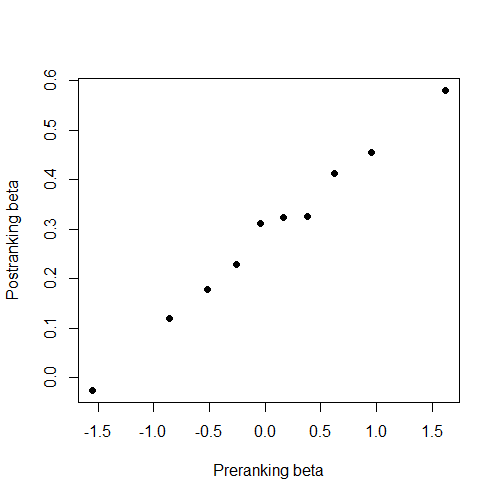
\includegraphics[width=0.70\textwidth]{Figure2.png}
\end{frame}





\begin{frame}{CID premium performance}
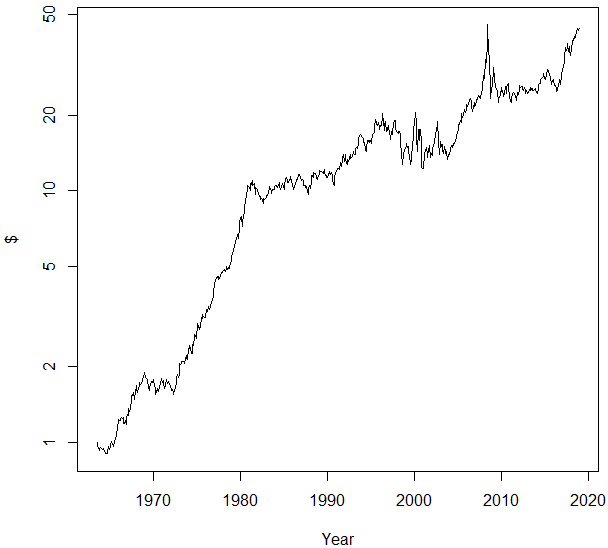
\includegraphics[width=0.70\textwidth]{Figure3.png}
\end{frame}




\begin{frame}{CID premium and industry coarseness}
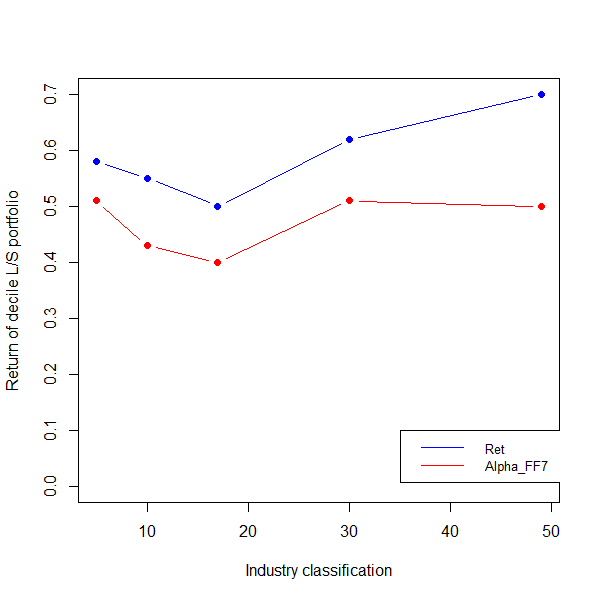
\includegraphics[width=0.70\textwidth]{alphas_inds.png}
\end{frame}



\begin{frame}{CID premium: doublesorts}
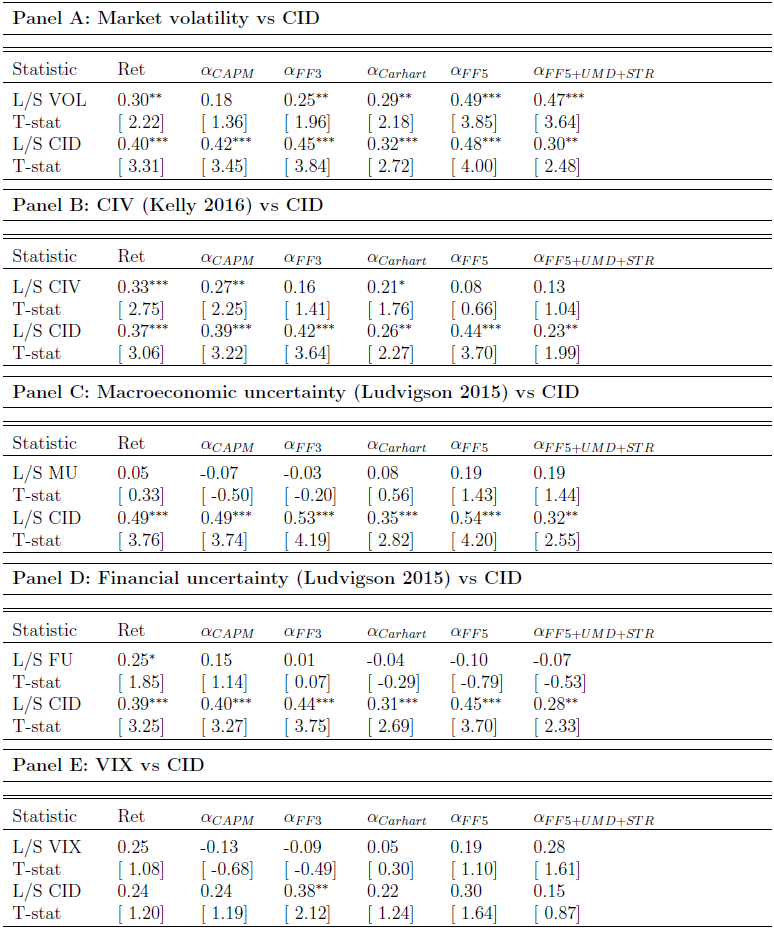
\includegraphics[width=0.56\textwidth]{doublesorts.png}
\end{frame}



\begin{frame}{CID from abnormal returns}
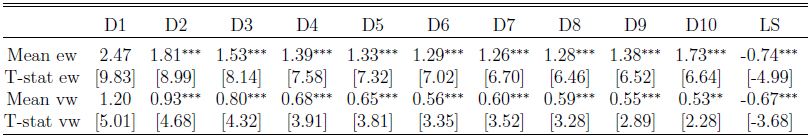
\includegraphics[width=1\textwidth]{cid_from_abns1.png} \\
\vspace{1cm}
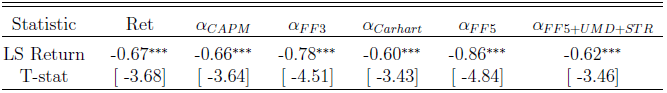
\includegraphics[width=1\textwidth]{cid_from_abns2.png}
\end{frame}




\end{document}

